\documentclass[a4paper]{article}


\usepackage[utf8]{inputenc}
\usepackage[german]{babel}
\usepackage{amsmath}
\usepackage{amssymb}
\usepackage{fancyhdr}
\usepackage{color}
\usepackage{graphicx}
\usepackage{lastpage}
\usepackage{listings} 
\usepackage{tikz}
\usepackage{pdflscape}
\usetikzlibrary{trees}
\usepackage{subfigure}
\usepackage{float}
\usepackage{polynom}
\usepackage{hyperref}
\usepackage{tabularx}
\usepackage{forloop}
\usepackage{geometry}
\usepackage{listings}
\usepackage[]{algorithm2e}
\usepackage{fancybox}
\usepackage{tikz}
\usetikzlibrary{shapes}

\usepackage{algorithmic}
\usetikzlibrary{automata,arrows}

\usepackage{xparse}
\input kvmacros

%Größe der Ränder setzen
\geometry{a4paper,left=3cm, right=3cm, top=3cm, bottom=3cm}

%Kopf- und Fußzeile
\pagestyle {fancy}
\fancyhead[L]{}
\fancyhead[C]{Datenbanksysteme}
\fancyhead[R]{\today}

\fancyfoot[L]{}
\fancyfoot[C]{}
\fancyfoot[R]{Seite \thepage /\pageref*{LastPage} }


%Formatierung der Überschrift, hier nichts ändern
\def\header#1#2{
\begin{center}
{\Large\bf Übungsblatt #1} %Blatt eintragen

{(Abgabetermin #2)}
\end{center}
}

%Definition der Punktetabelle, hier nichts ändern
\newcounter{punktelistectr}
\newcounter{punkte}
\newcommand{\punkteliste}[2]{%
  \setcounter{punkte}{#2}%
  \addtocounter{punkte}{-#1}%
  \stepcounter{punkte}%<-- also punkte = m-n+1 = Anzahl Spalten[1]
  \begin{center}%
  \begin{tabularx}{\linewidth}[]{@{}*{\thepunkte}{>{\centering\arraybackslash} X|}@{}>{\centering\arraybackslash}X}
      \forloop{punktelistectr}{#1}{\value{punktelistectr} < #2 } %
      {%
        \thepunktelistectr & 
      } 
      #2 &  $\Sigma$ \\
      \hline
      \forloop{punktelistectr}{#1}{\value{punktelistectr} < #2 } %
      {%
        &
      } &\\ 
      \forloop{punktelistectr}{#1}{\value{punktelistectr} < #2 } %
      {%
        &
      } &\\ 
    \end{tabularx}
  \end{center}
}



\begin{document}

%Hier bitte Student 1 usw ersetzen
\begin{tabularx}{\linewidth}{m{0.2 \linewidth}X}
\begin{minipage}{\linewidth}%
%
% ----------------------- TODO ---------------------------
%Hier Namen eintragen
%
Marc Tomasek \\
Marius Hobbhahn \\
\end{minipage} & \begin{minipage}{\linewidth}%
%
% ----------------------- TODO ---------------------------
%Die zweite Zahl durch die Anzahl der Aufgaben ersetzen
%
%
\punkteliste{1}{3} %
%
\end{minipage}\\
\end{tabularx}



% ----------------------- TODO ---------------------------
%
%Hier Nummer und Datum aktualisieren
\header{Nr. 10}{17.01.2018}
%---------------------------------------------------------------------------
\section*{1 - Cartographic coloring}
\subsection*{a - Graph without Solution}
\begin{center}
	\begin{tikzpicture}[scale=0.2]
	\tikzstyle{every node}+=[inner sep=0pt]
	\draw [black] (21.8,-10.8) circle (3);
	\draw (21.8,-10.8) node {$A$};
	\draw [black] (42.6,-10.8) circle (3);
	\draw (42.6,-10.8) node {$B$};
	\draw [black] (42.6,-28.3) circle (3);
	\draw (42.6,-28.3) node {$D$};
	\draw [black] (21.4,-28.3) circle (3);
	\draw (21.4,-28.3) node {$C$};
	\draw [black] (39.6,-10.8) -- (24.8,-10.8);
	\draw [black] (21.73,-13.8) -- (21.47,-25.3);
	\draw [black] (24.4,-28.3) -- (39.6,-28.3);
	\draw [black] (42.6,-25.3) -- (42.6,-13.8);
	\draw [black] (40.29,-12.71) -- (23.71,-26.39);
	\draw [black] (24.1,-12.73) -- (40.3,-26.37);
\end{tikzpicture} \\ 
	\begin{tabular}{l || c | c | c | c }
	assignment & A & B & C & D \\ \hline
	init & rgb & rgb & rgb & rgb  \\
	A $\leftarrow$ r & r & gb & gb & gb \\
	B $\leftarrow$ g & r & g & b & b \\
	C $\leftarrow$ b & r & g & b & * \\
	B $\leftarrow$ b & r & b & g & g \\
	C $\leftarrow$ g & r & b & g & ** \\
	A $\leftarrow$ g & g & rb & rb & rb \\
	B $\leftarrow$ r & g & r & b & b  \\
	C $\leftarrow$ b & g & r & b & *** \\
	B $\leftarrow$ b & g & b & r & r \\
	C $\leftarrow$ r & g & b & r & **** \\
	A $\leftarrow$ b & b & rg & rg & rg \\
	B $\leftarrow$ r & b & r & g & g \\
	C $\leftarrow$ g & b & r & g & ***** \\
	B $\leftarrow$ g & b & g & r & r \\
	C $\leftarrow$ r & b & g & r & ****** \\
\end{tabular} \\
	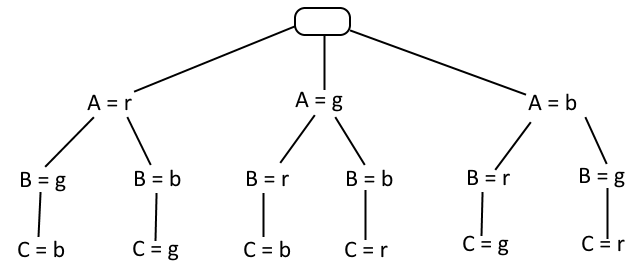
\includegraphics[scale=0.5]{tree.png} \\
\end{center}
In situations with an odd number of stars, we track back to the previous assignment of b and switch that. In situations with an even number of stars we track back to the assignment of A and switch this. When having 6 stars we reached all possible assigments of A in combination with others and realized that there is no consistent assigment.

\subsection*{b - Less than 6 Edges}
We can't construct a graph with 4 nodes and 5 edges, which does not admit a solution: \\
The CSP-graph from \textit{a} is fully connected. If we now remove one edge, we remove a connection between two nodes and the graph is not fully connected anymore. Because these two nodes do not share a constraint, they can be colored in with the same color:
\begin{center}
	\begin{tikzpicture}[scale=0.2]
		\tikzstyle{every node}+=[inner sep=0pt]
		\draw [black] (9.5,-6.3) circle (3);
		\draw [black] (23.8,-6.3) circle (3);
		\draw (23.8,-6.3) node {$r$};
		\draw [black] (9.5,-20.9) circle (3);
		\draw [black] (23.8,-20.9) circle (3);
		\draw (23.8,-20.9) node {$r$};
		\draw [black] (11.6,-8.44) -- (21.7,-18.76);
		\draw [black] (9.5,-9.3) -- (9.5,-17.9);
		\draw [black] (12.5,-20.9) -- (20.8,-20.9);
		\draw [black] (12.5,-6.3) -- (20.8,-6.3);
		\draw [black] (11.6,-18.76) -- (21.7,-8.44);
	\end{tikzpicture}
\end{center}
To find a solution, simply color the remaining two nodes in differing colors, except the one we chose earlier.
\begin{center}
	\begin{tikzpicture}[scale=0.2]
		\tikzstyle{every node}+=[inner sep=0pt]
		\draw [black] (9.5,-6.3) circle (3);
		\draw ((9.5,-6.3) node {$g$};
		\draw [black] (23.8,-6.3) circle (3);
		\draw (23.8,-6.3) node {$r$};
		\draw [black] (9.5,-20.9) circle (3);
		\draw (9.5,-20.9) node {$b$};
		\draw [black] (23.8,-20.9) circle (3);
		\draw (23.8,-20.9) node {$r$};
		\draw [black] (11.6,-8.44) -- (21.7,-18.76);
		\draw [black] (9.5,-9.3) -- (9.5,-17.9);
		\draw [black] (12.5,-20.9) -- (20.8,-20.9);
		\draw [black] (12.5,-6.3) -- (20.8,-6.3);
		\draw [black] (11.6,-18.76) -- (21.7,-8.44);
	\end{tikzpicture}
\end{center}
This will always lead to a consistent solution in which it does not matter which edge was removed in the first place. \\ \\

\section*{2 - n-Queens Problem}
\subsection*{a}
In the Group of $n$ Variables $X = \{X_1, X_2, ... X_n\}$, each variable represents the placement of one queen in the column $X_i$.

\subsection*{b}
$X_1$ for example represents the first column. The $n$ possible values range from $1 \leq i \leq n, i \in \mathbb{N}$ which represent the placement of the queen in that column.

\begin{center}
	\includegraphics*[]{schach.png}
\end{center}

\subsection*{c}
We will find no vertical conflicts due to our variable definition, so we don't need to define constraints for them. \\
Horizontal conflicts, can be checked for by $AllDiff(X)$.
\begin{itemize}
	\item Diagonal conflicts to the right of our current piece $X_i$: \\
		$X_i + (k-i) \neq X_k, \\
		 X_i - (k-i) \neq X_k, 		\quad \forall k \in \mathbb{N}: i < k \leq n$
	\item Diagonal conflicts to the left of our current piece $X_i$: \\
		$X_i + (i-f) \neq X_f, \\
		 X_i - (i-f) \neq X_f, 		\quad \forall f \in \mathbb{N}: 1 \leq f < i$
\end{itemize}

\section*{3 - Heuristics and consistency}
\subsection*{a}
forward checking: It begins by assigning the first value of possible values for variables to the first node in the graph (assuming that an order is given) and propagates the logical results of that assignments to neighboring nodes to remove possible values of their set of values. If an inconsistency is found it is solved through backtracking. The main difference to MAC is that it only looks at neighboring nodes and not the whole graph at any given point in time\\
Maintaining arc consistency (MAC): It begins by assigning the first value of possible values for variables to the first node in the graph (assuming that an order is given) then tests all constraints with neighboring nodes and removes possible values from their set of values until every arc in the graph fulfills the criterion of arc consistency. If an inconsistency is found it is solved through backtracking. The main difference to forward checking is that with MAC we check the whole graph for consistency not only the neighboring nodes of the current variable.

\subsection*{b}
We choose the variable that is most constrained to remove as many constraints as possible from any further inquiry because that makes following solutions easier. \\
We choose the value with least constraints so that we can fulfill as many constraints as possible and make following solutions easier.

\subsection*{c}
A variable is arc consistent with another variable if there are admissible combinations of values between the two, meaning that there is at least one combination of admissible assigment for the second variable for each admissible assigment of variable 1. \\
A variable is path consistent with a third variable if each admissible assignment for variable one can be extended to the third variable. That means every binary constraint on the path between variable one and three are fullfilled with admissible assignments.

\end{document}